We present results in two parts.
We open with the fair coin case ($\theta_{\rm true}=\theta_{\rm null}=0.5$):
a hand-picked experiment to illustrate the qualitative behaviour of all three algorithms
(Section~\ref{sec:fair_coin_sequence}), followed by a large-scale study across
$M=5{,}000$ independent experiments (Section~\ref{sec:fair_coin_large_scale}) and a
sensitivity analysis over the precision goal $\omega_{\rm goal}$
(Section~\ref{sec:goal_impact}).
We then examine how all three algorithms perform as $\theta_{\rm true}$ increases from
$0.5$ upwards, across and beyond the ROPE (Section~\ref{sec:trends}).

\subsection{Fair Coin ($\theta_{\rm true}=0.5$)}\label{sec:fair_coin}

\subsubsection{A Hand-Picked Sequence}\label{sec:fair_coin_sequence}

Figure~\ref{fig:iterations} presents a hand-picked randomly generated fair coin experiment chosen to
illustrate contrasting outcomes across the three algorithms.\footnote{This figure is similar to the top
panels in \cite{kruschke2015doing} Figures 13.4 and 13.5.}
(note that all performance claims rest on the large-scale simulation study of
Section~\ref{sec:fair_coin_large_scale})
The posteriors in Figure~\ref{fig:posteriors} correspond to three specific iterations
of this same experiment.\footnote{The sequence may be found in the open-source material
as \href{https://github.com/elzurdo/precision-goal/blob/main/py/utils_experiments.py\#L28}{\texttt{SEQUENCE\_HANDPICKED}}.}

Despite arising from the same sequence of coin tosses, the three algorithms reach
sharply different decisions.
The HDI+ROPE algorithm stops early at iteration 126 (vertical red dashed line) and, incorrectly,
rejects $\theta_{\rm null}$.
PitG stops at iteration 598 (first purple dot, where the precision goal is first met)
but is left inconclusive, as the HDI straddles the ROPE boundary.
DPitG waits until both conditions are jointly satisfied, stopping at iteration 804
(first green solid line coinciding with a purple dot) and correctly accepts
$\theta_{\rm null}$.
This divergence from a single experiment motivates the large-scale analysis that
follows.

\begin{figure}[h!]
  \centering
  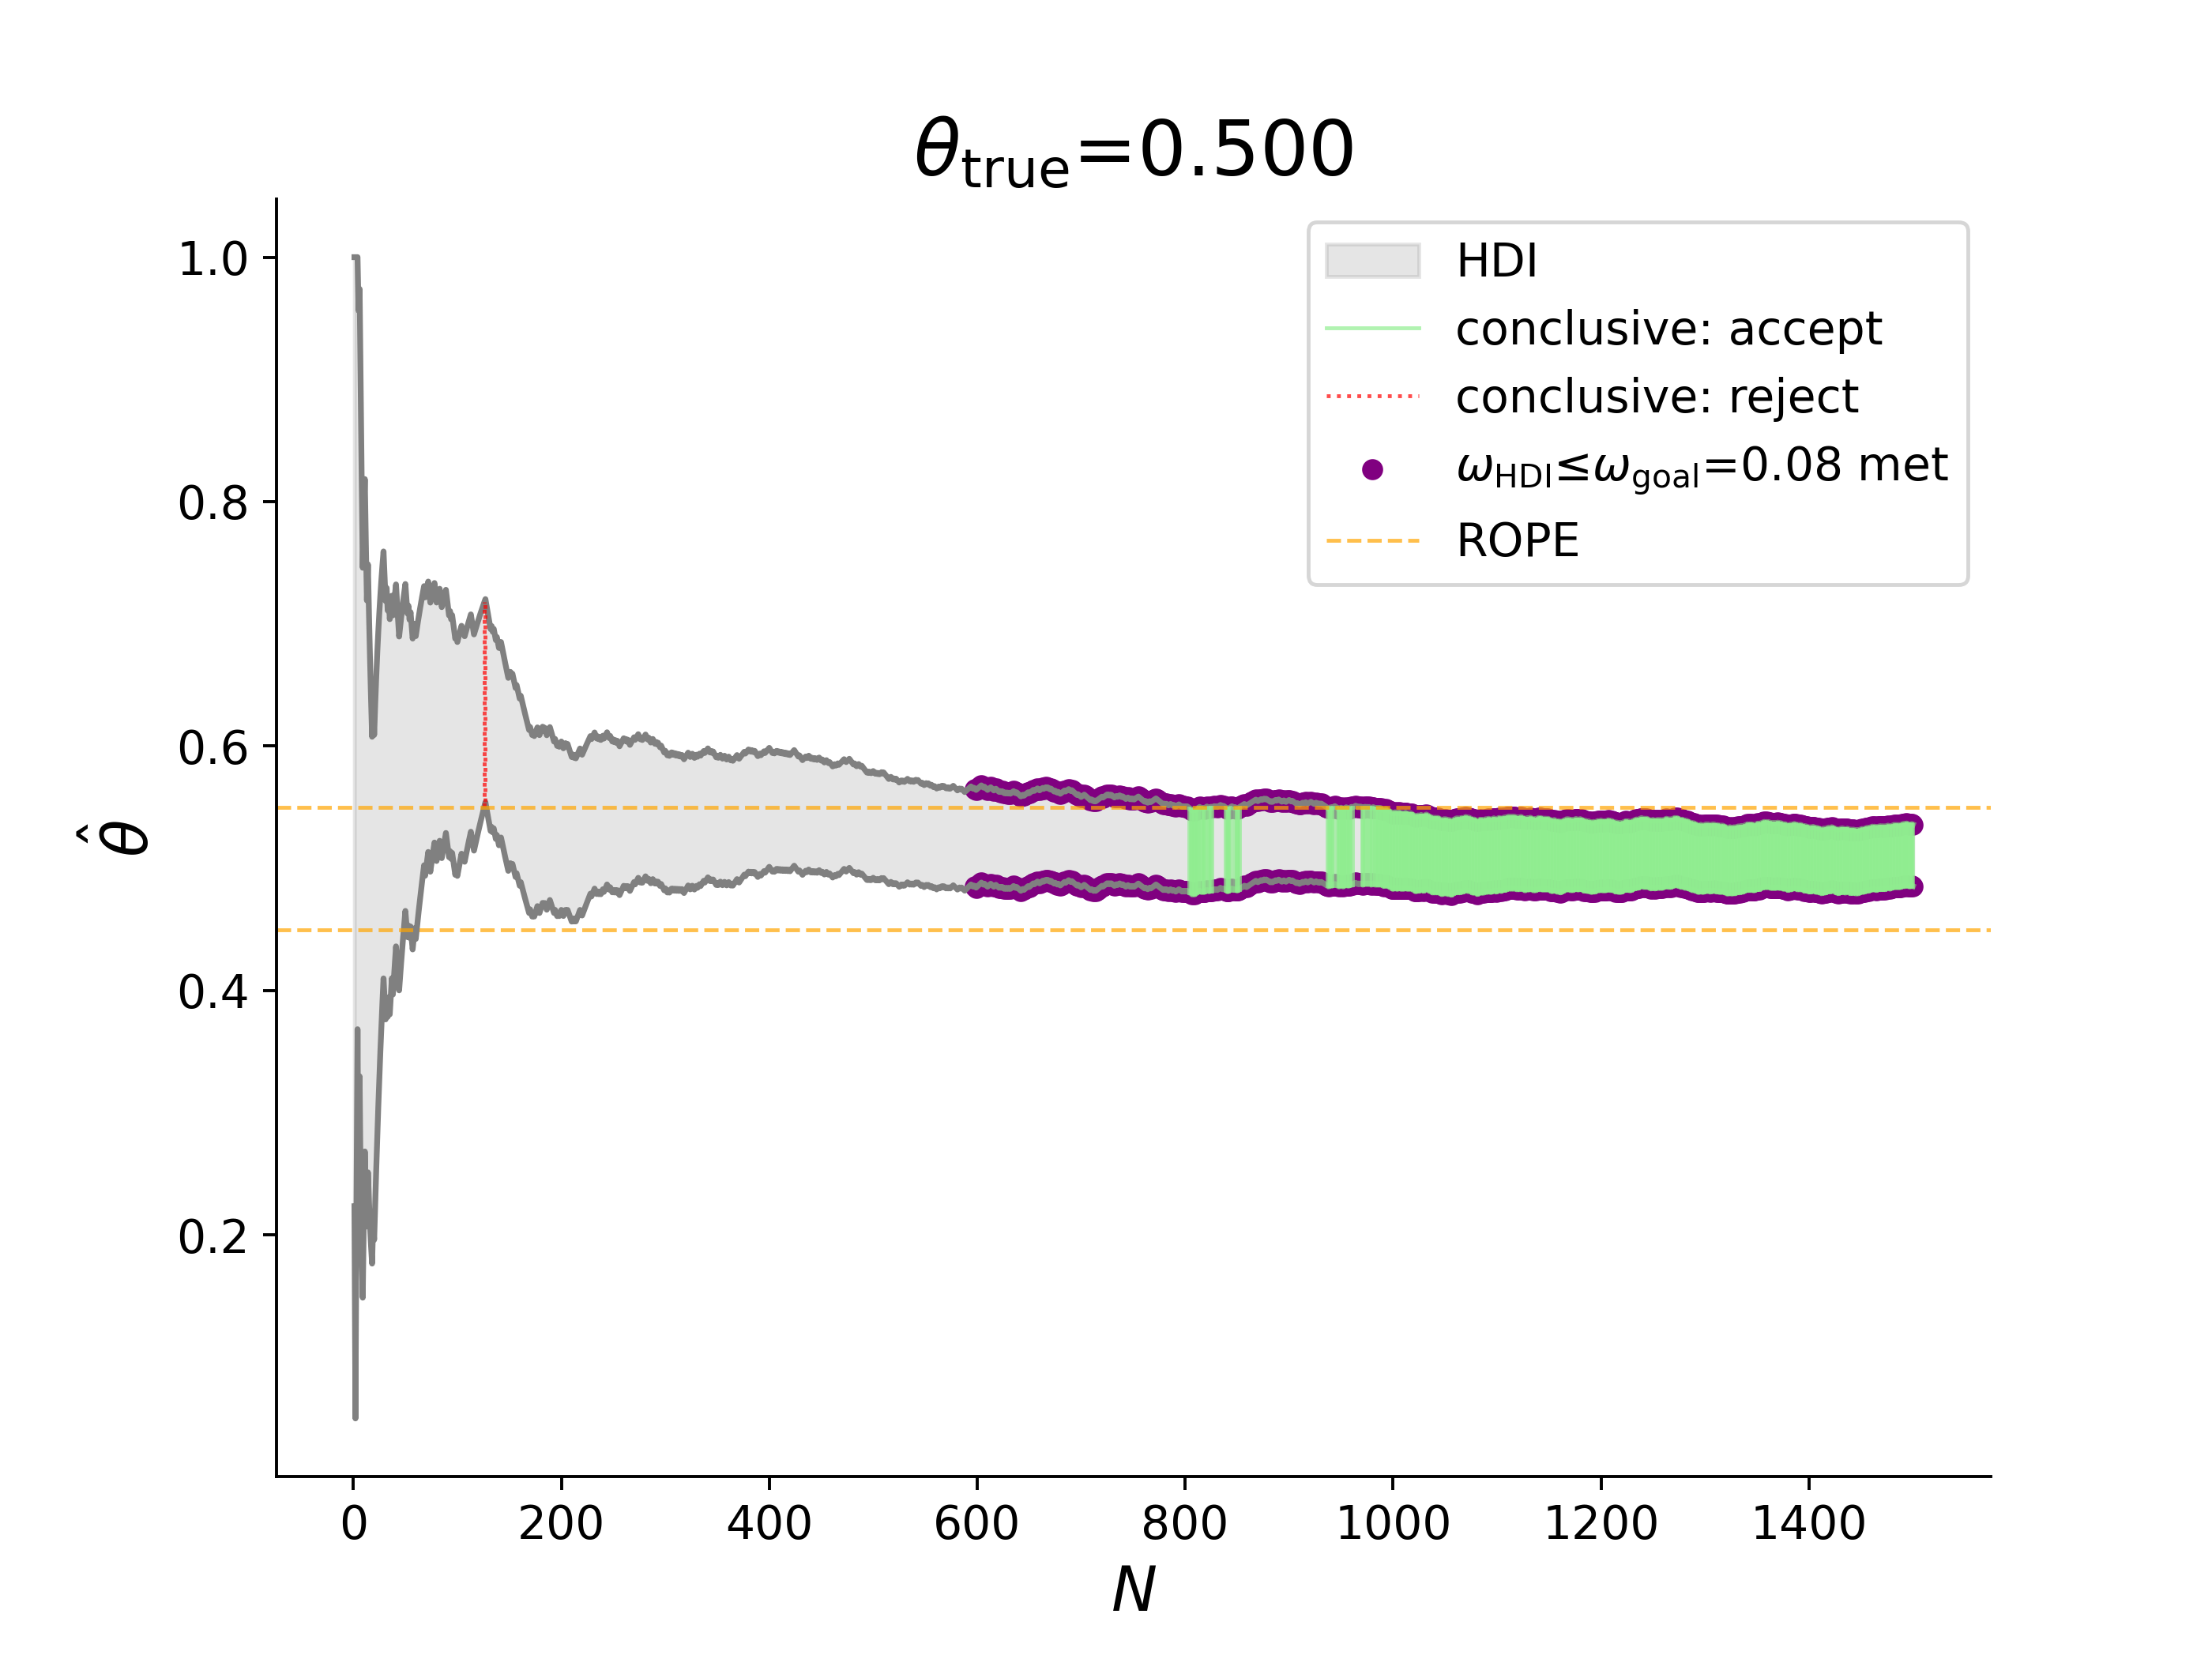
\includegraphics[width=1\textwidth]{handpicked_sequence_stats_dpi350.png}
  \caption{Cumulative sample proportion $\hat{\theta}(N)$ at each iteration $N$ of a
  hand-picked randomly generated fair coin experiment
  ($\theta_{\rm true}=\theta_{\rm null}=0.5$, $\omega_{\rm goal}=0.08$, $N_{\rm min}=30$)
  illustrating varied outcomes across sampling.
  $\hat{\theta}(N)$ denotes the observed proportion of successes (heads) in $N$ trials.
  \textit{Gray band}: 95\% HDI of the posterior; its width is $\omega_{\rm HDI}$.
  \textit{Horizontal dashed lines}: ROPE boundaries.
  \textit{Vertical red dashed line}: Decision to reject $\theta_{\rm null}$.
  \textit{Vertical green solid line}: Decision to accept $\theta_{\rm null}$.
  \textit{Purple dots}: Precision goal met ($\omega_{\rm HDI} \le \omega_{\rm goal}$).
  See Figure~\ref{fig:posteriors} for the posterior distributions at the three marked
  stop iterations.}
  \label{fig:iterations}
\end{figure}

\subsubsection{Large-Scale Experiments}\label{sec:fair_coin_large_scale}

We expand this analysis to $M=5{,}000$ experiments, displaying outcomes in
Figures~\ref{fig:fair_iter_vs_rate} and~\ref{fig:fair_decisions},\footnote{Both of these
visuals are inspired by Figure~13.6 of \cite{kruschke2015doing}.} and summarising key
statistics in Tables~\ref{tab:fair_overall} and~\ref{tab:fair_conclusive}.

\begin{figure}[h!]
  \centering
  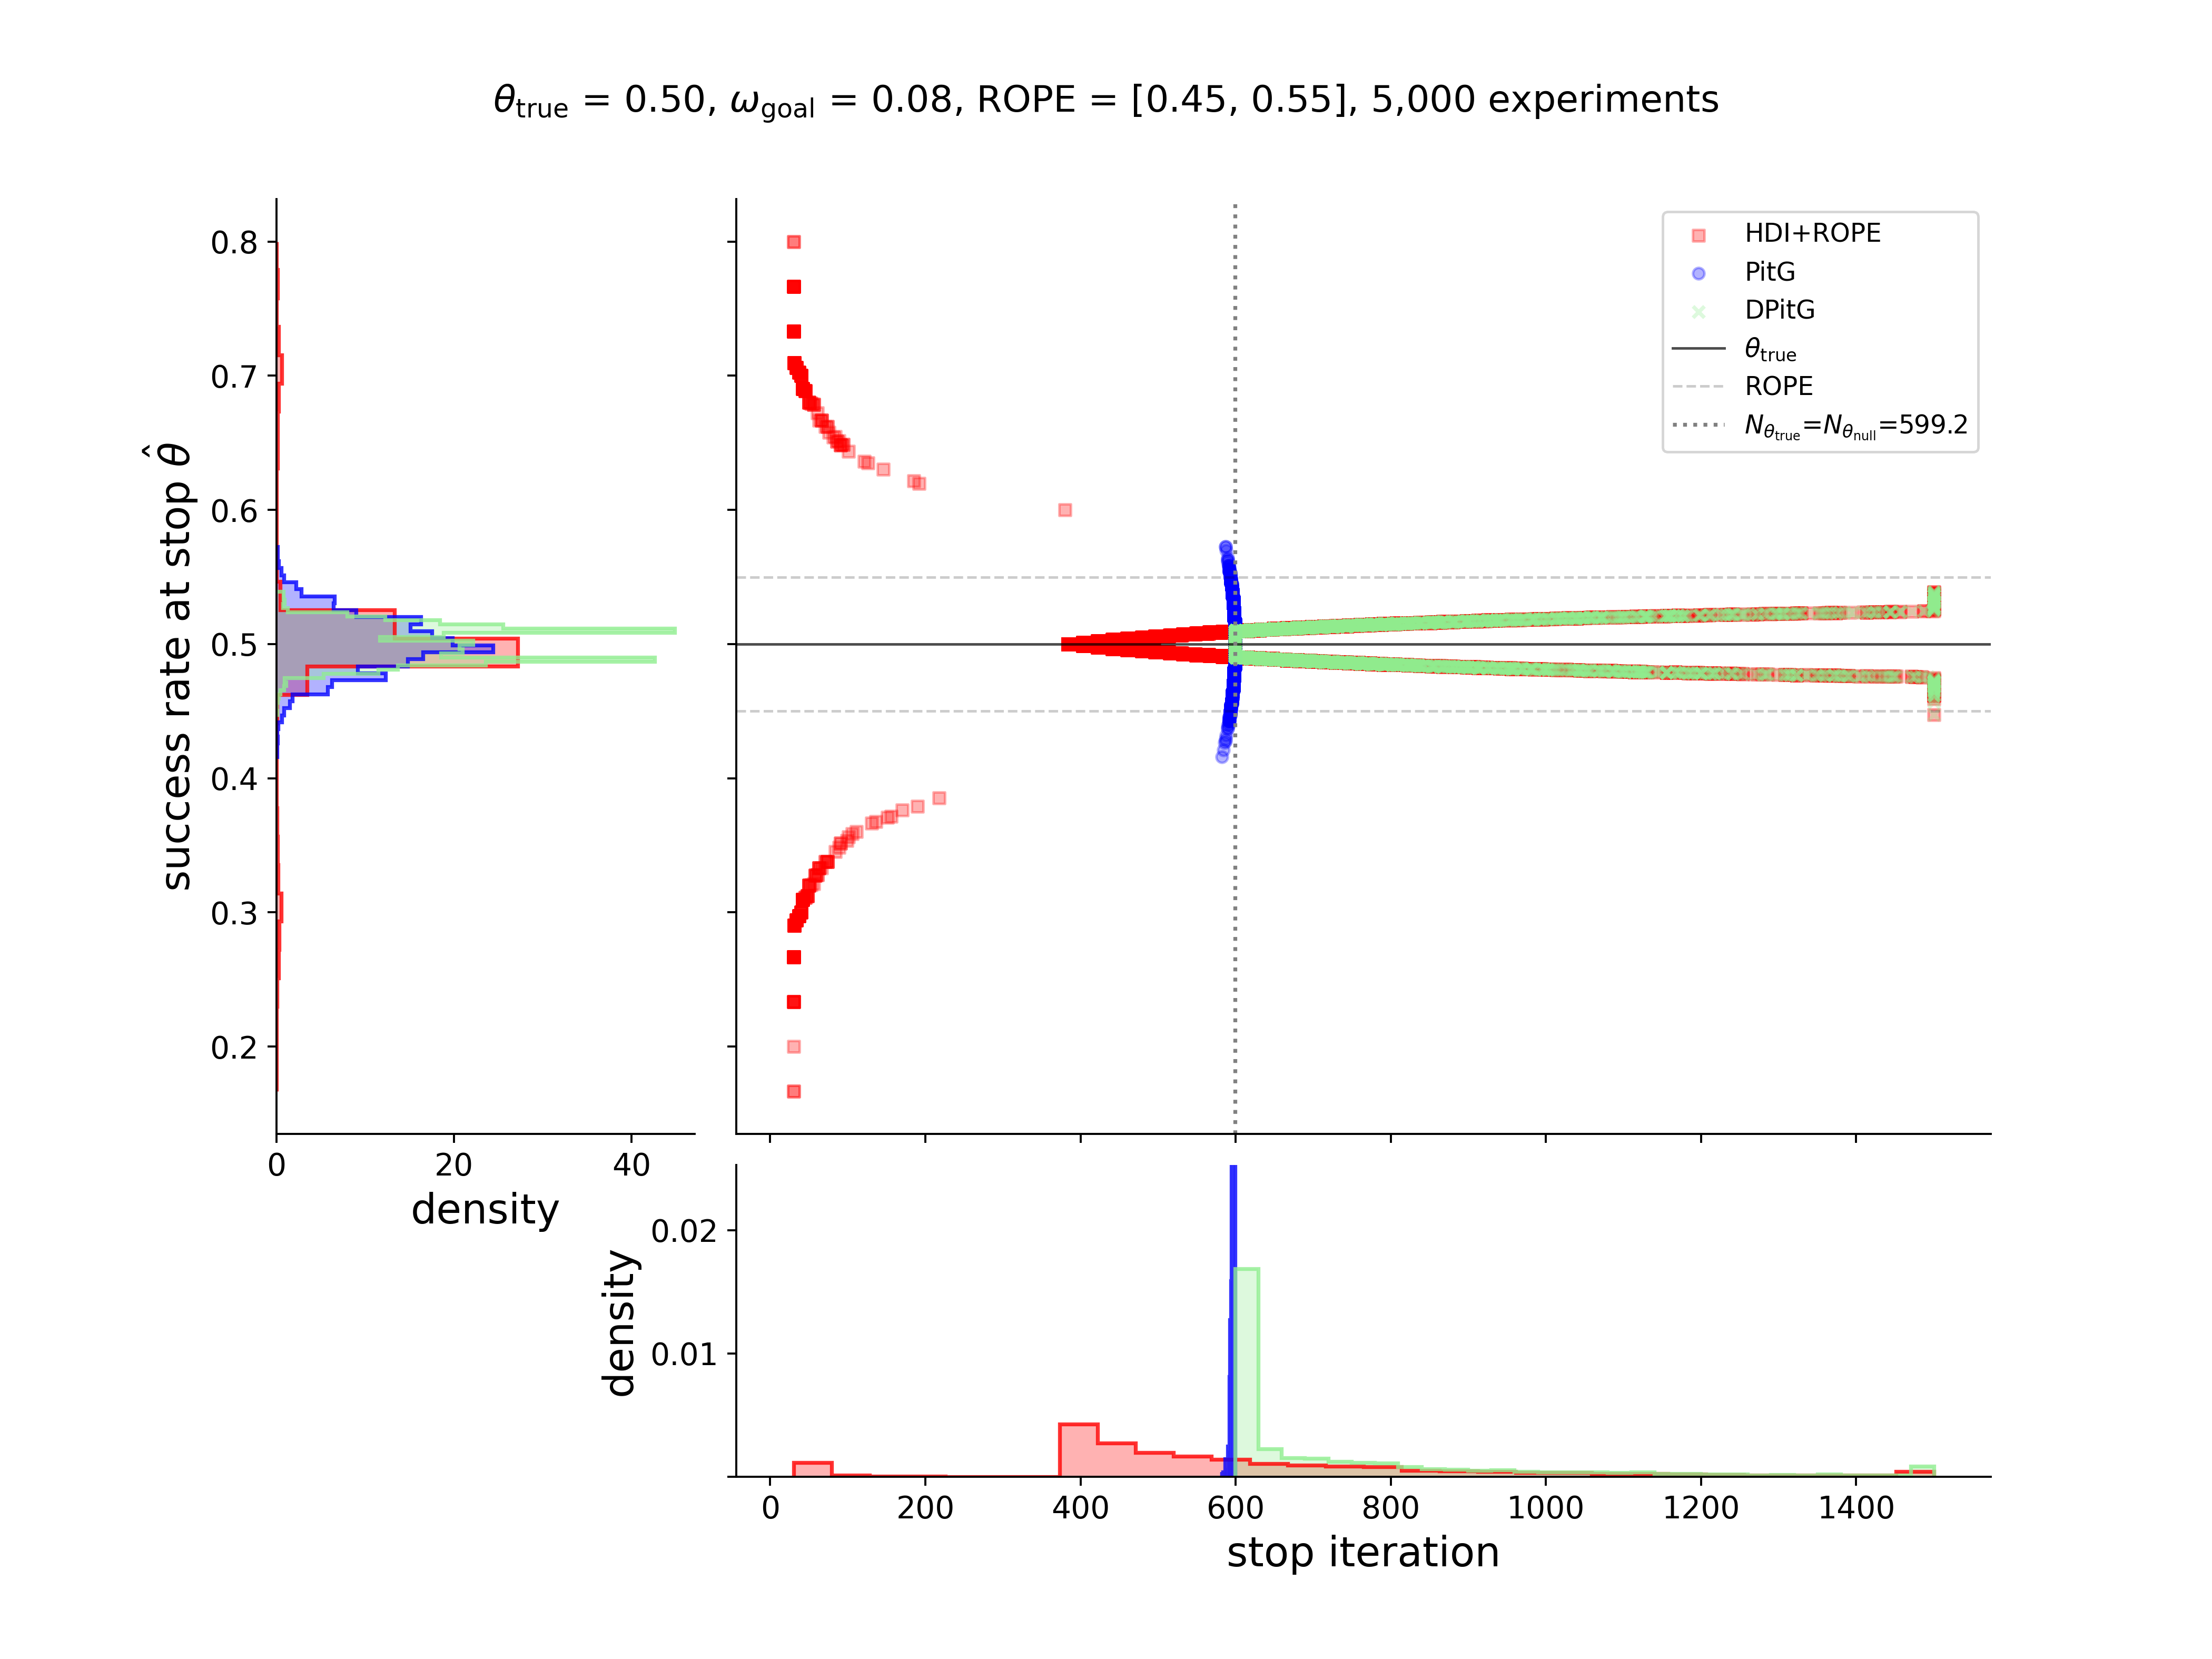
\includegraphics[width=1\textwidth]{faircoin_nstop_successrate_dpi350.png}
  \caption{Outcomes of $M=5{,}000$ fair coin experiments ($\theta_{\rm true}=\theta_{\rm null}=0.5$,
  $\omega_{\rm goal}=0.08$, $N_{\rm min}=30$).
  \textit{Main panel}: scatter plot of sample proportion $\hat{\theta}(N_{\rm stop})$
  vs.\ stop iteration $N_{\rm stop}$.
  \textit{Symbols}: red squares: HDI+ROPE; blue circles: PitG; green Xs: DPitG.
  \textit{Solid horizontal line}: $\theta_{\rm true}$.
  \textit{Horizontal dashed lines}: ROPE boundaries.
  \textit{Vertical dashed line}: expected goal stop iteration $N_{\rm goal}$
  (Equation~\ref{eq:pitg_stop_iteration}); here $N_{\rm goal}(\theta_{\rm true})=
  N_{\rm goal}(\theta_{\rm null})$ since $\theta_{\rm true}=\theta_{\rm null}$.
  \textit{Bottom panel}: histograms of $N_{\rm stop}$.
  \textit{Left panel}: histograms of $\hat{\theta}(N_{\rm stop})$.
  The marginal histograms reveal where most results concentrate,
  complementing the scatter plot which shows the correlations.
  Histogram binning varies by algorithm to best resolve each distribution.}
  \label{fig:fair_iter_vs_rate}
\end{figure}

Figure~\ref{fig:fair_iter_vs_rate} shows that the HDI+ROPE algorithm yields a wide range of stop
iterations and sample proportions $\hat{\theta}$, with a non-negligible proportion
of results falling outside the ROPE ($\hat{\theta}$ ranging from $\sim\!0.25$ to
$\sim\!0.80$), leading to incorrect rejections
of $\theta_{\rm null}$. Its $N_{\rm stop}$ distribution is skewed towards early stopping
at $\sim\!400$, well before $N_{\rm goal}\sim 600$, with a long tail extending to later
iterations.

PitG consistently stops near $N_{\rm goal}$, with sample proportions clustered tightly around
$\theta_{\rm true}=0.5$. However, many of these stops occur when the HDI straddles the
ROPE boundary, yielding a high rate of inconclusive decisions
(see Figure~\ref{fig:fair_decisions} and Table~\ref{tab:fair_overall}).
DPitG exhibits a narrower $\hat{\theta}(N_{\rm stop})$ distribution than PitG but extends
to later iterations, achieving more conclusive results while maintaining zero estimation bias.\footnote{
In Section~\ref{sec:trends} we demonstrate that some bias emerges as symmetry breaks.}
The $N_{\rm stop}$ histograms in Figure~\ref{fig:fair_iter_vs_rate} make this concrete:
DPitG's distribution begins near $N_{\rm goal}$, precisely where PitG's terminates,
confirming the structural equivalence noted in
Section~\ref{sec:expected_stop_iteration}: DPitG behaves as the HDI+ROPE algorithm with
$N_{\rm min} \approx N_{\rm goal}$ rather than a fixed small floor.


\begin{figure}[h!]
  \centering
  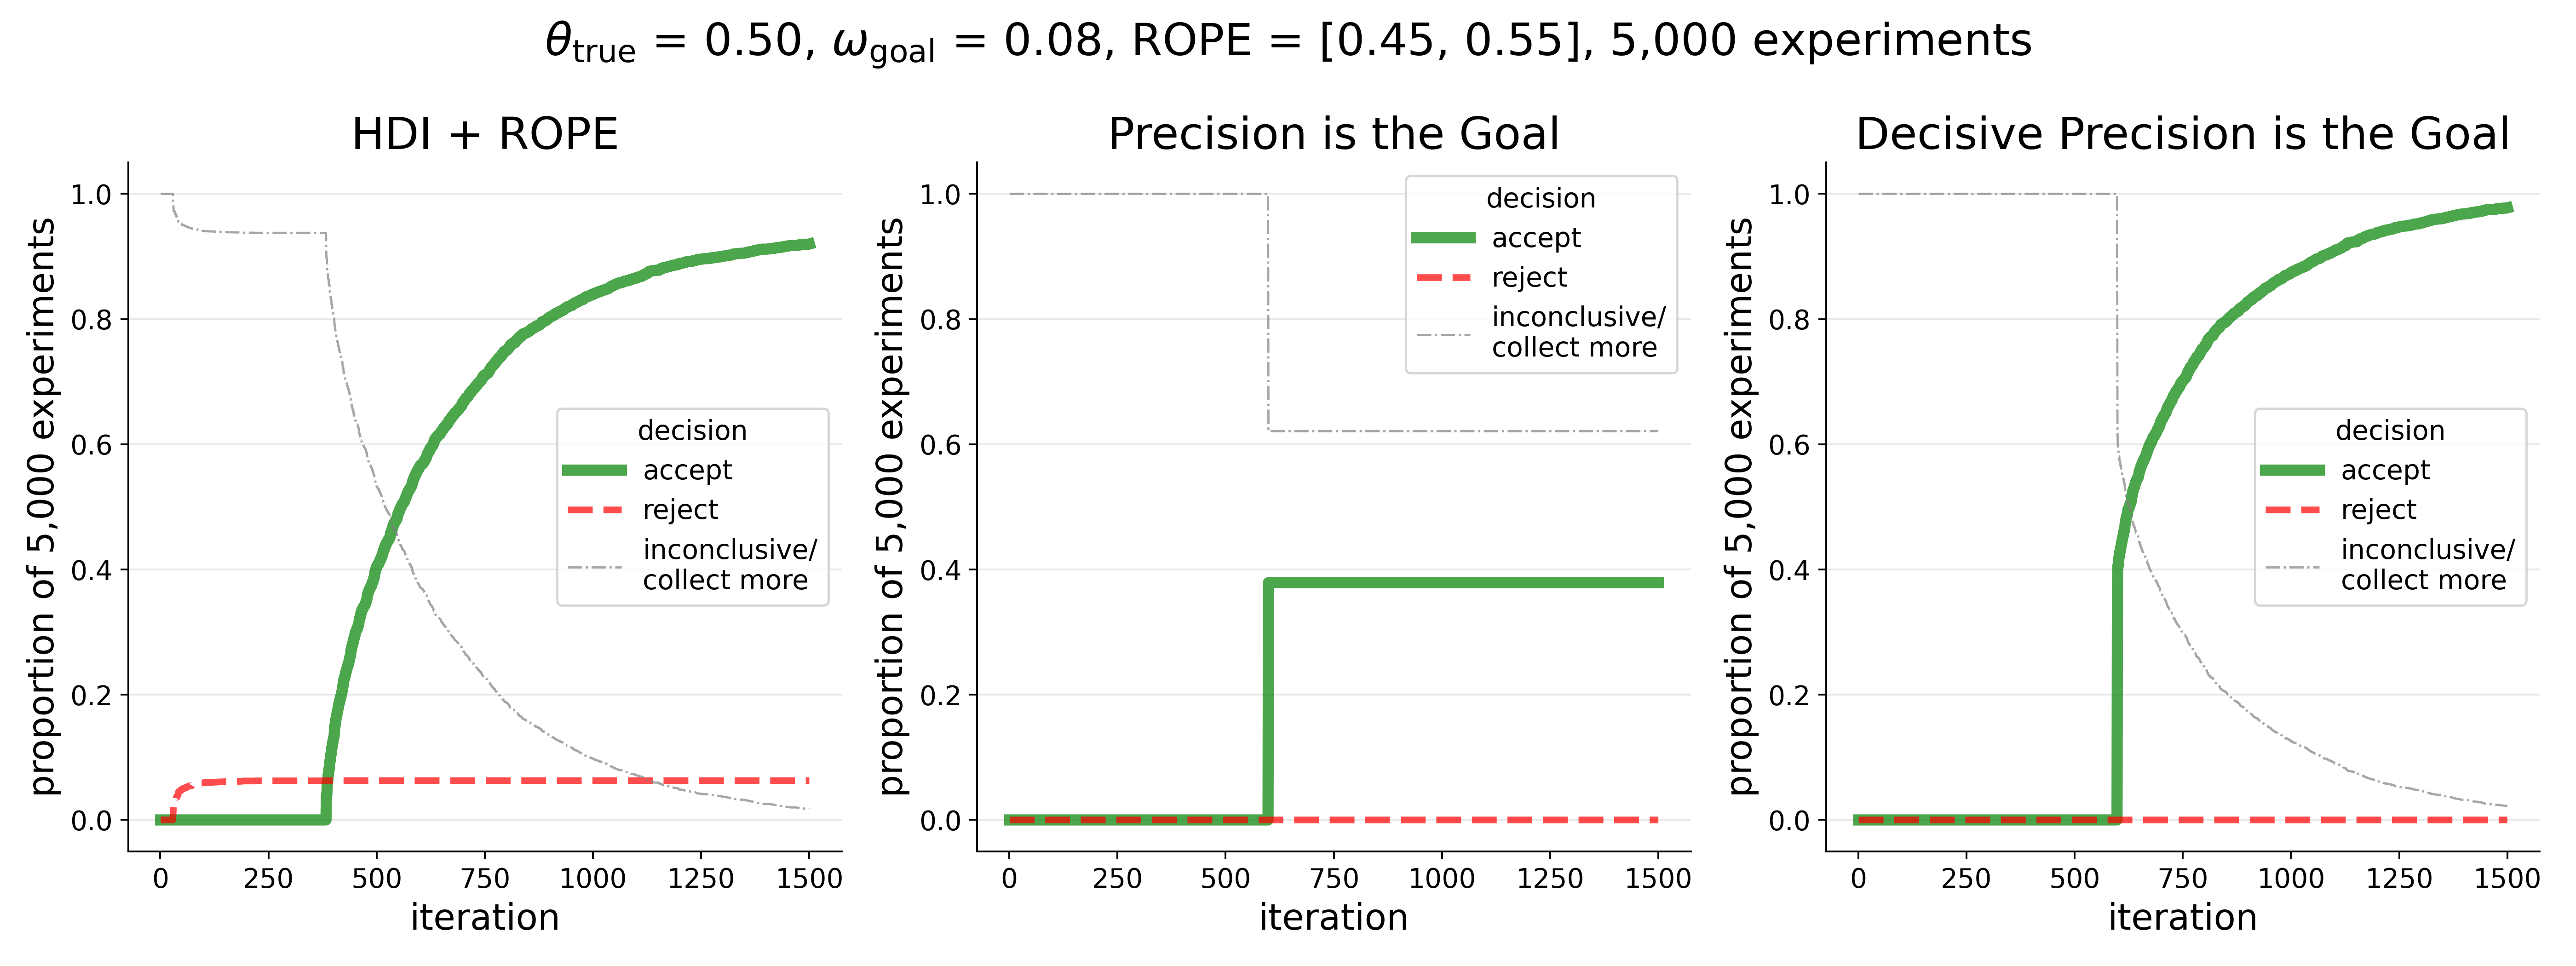
\includegraphics[width=1\textwidth]{faircoin_decision_rates_dpi350.png}
  \caption{Cumulative decision rates across iterations for $M=5{,}000$ fair coin experiments
  ($\theta_{\rm true}=\theta_{\rm null}=0.5$, $\omega_{\rm goal}=0.08$, $N_{\rm min}=30$).
  At each iteration $N$, the plotted proportions count all experiments that reached
  a decision at or before $N$; their sum is 100\% at every point.
  \textit{Left}: HDI+ROPE; \textit{Middle}: Precision is the Goal; \textit{Right}: Decisive Precision is the Goal.
  \textit{Red dashed line}: reject $\theta_{\rm null}$.
  \textit{Green solid line}: accept $\theta_{\rm null}$.
  \textit{Gray dot-dashed line}: inconclusive.}
  \label{fig:fair_decisions}
\end{figure}

Figure~\ref{fig:fair_decisions} shows that the HDI+ROPE algorithm's rejection rate (left panel) quickly asymptotes to 6\%, while its acceptance
rate begins rising near $N\sim 400$, reflecting a gradual shift from incorrect rejections
to correct acceptances as more data accumulate.

Both precision-based methods maintain a zero rejection rate (middle and right panels),
as they require the precision criterion to be satisfied before any decision is made.
For PitG (middle panel), the acceptance rate rises as a near step-function, jumping at
$N_{\rm goal}$ to 37.9\%, with the inconclusive rate settling at the complement 62.1\%.

DPitG (right panel) presents a hybrid of the other two: it preserves the zero-rejection
property of PitG while achieving a high conclusiveness rate akin to the HDI+ROPE algorithm, but with
a more gradual transition from inconclusive to conclusive outcomes.

Table~\ref{tab:fair_overall} summarises stop-iteration statistics across all $M$ experiments;
Table~\ref{tab:fair_conclusive} then restricts to the conclusive subsets and breaks outcomes
into acceptance and rejection rates alongside the $\hat{\theta}$ distribution at stop.

\begin{table}[h!]
  \begin{center}
  \begin{tabular}{c|c|c|c|c}
    \hline
    Algorithm &  Conclusive Rate  & $N_{\rm 50\%}$ & $N_{\rm 25\%}$--$N_{\rm 75\%}$ & $\Delta_{\rm IQR}$\\
    \hline
    HDI+ROPE & 0.982 & 521 & 415 - 723& 308  \\
    PitG     & \textcolor{red}{\textbf{0.379}}  & 599 & 598 - 599& 1 \\
    DPitG    & \textcolor{green}{\textbf{0.978}}  & 627 & 598 - 794& 196 \\
    \hline
  \end{tabular}
  \caption{Summary statistics for all $M=5{,}000$ fair coin experiments
  ($\theta_{\rm true}=\theta_{\rm null}=0.5$, $\omega_{\rm goal}=0.08$, $N_{\rm min}=30$;
  cf.\ Figure~\ref{fig:fair_iter_vs_rate}).
  $N_{\rm 50\%}$: median stop iteration;
  $N_{\rm 25\%}$--$N_{\rm 75\%}$: interquartile range of stop iteration.
  Conclusive Rate values are color-coded: \textcolor{red}{\textbf{red}} flags a
  concerningly low rate (PitG); \textcolor{green}{\textbf{green}} highlights DPitG's
  strong rate with zero false rejections (cf.\ Table~\ref{tab:fair_conclusive}).}
  \label{tab:fair_overall}
\end{center}
\end{table}

The HDI+ROPE algorithm achieves the highest conclusiveness rate (98.2\%), but at the cost of a 6.3\%
false-reject rate. PitG delivers zero false rejections, but its conclusiveness rate of
only 37.9\% is strikingly low, with stop iterations all clustering at $N_{\rm goal}$.
DPitG delivers the balance sought in Section~\ref{sec:decisive_pitg}: a 97.8\%
conclusiveness rate with zero false
rejections. The lower quartile ($N_{\rm 25\%}=598$) nearly equals $N_{\rm goal}=599$,
confirming that a substantial fraction of DPitG experiments stop as soon as the
precision goal is first met; the wider IQR of $598$--$794$ reflects those that
require additional iterations to satisfy the joint precision-and-conclusiveness
criterion, at a median cost of only 4.7\% more samples across all $M$ experiments
(4\% when restricted to conclusive experiments; see Table~\ref{tab:fair_conclusive})
than PitG.


\begin{table}[h!]
  \begin{center}
  \begin{tabular}{c|c|c|c|c|c}
    \hline
    Algorithm & Conclusive & Acceptance Rate & Rejection Rate &  $\hat{\theta}_{\rm 50\%}$ & $\hat{\theta}_{\rm 25\%} - \hat{\theta}_{\rm 75\%}$\\
    \hline
    HDI+ROPE & 4912 & 0.936 & \textcolor{red}{\textbf{0.064}} & 0.5000 & 0.4920-0.5081 \\
    PitG     &  \textbf{1895} & 1     & 0     & 0.5008 & 0.4958-0.5041 \\
    DPitG    & 4888 & 1     & 0     & 0.5008 & 0.4895-0.5105\\
    \hline
  \end{tabular}
  \caption{Summary statistics for the conclusive subsets of experiments in
  Table~\ref{tab:fair_overall}.
  Conclusive: count of experiments (out of 5{,}000) with a conclusive outcome.
  Acceptance and Rejection rates are conditioned on conclusive experiments
  and therefore sum to 1.
  $\hat{\theta}_{\rm 50\%}$: median sample proportion at stop;
  $\hat{\theta}_{\rm 25\%} - \hat{\theta}_{\rm 75\%}$: interquartile range of
  sample proportion at stop.
  \textcolor{red}{\textbf{Red}} flags a non-zero false-reject rate (HDI+ROPE); \textbf{bold} flags a concerningly low conclusive count (PitG).}
  \label{tab:fair_conclusive}
\end{center}
\end{table}

\subsubsection{Sensitivity to $\omega_{\rm goal}$}\label{sec:goal_impact}

The choice of $\omega_{\rm goal}$ governs the fundamental precision--conclusiveness
trade-off for PitG. Table~\ref{tab:goal_impact} shows the effect across a range of values
at $\theta_{\rm true}=0.5$. Tightening $\omega_{\rm goal}$ (decreasing it) raises PitG's
conclusiveness at the cost of a larger required sample size: $N_{\rm goal}$ grows
quadratically as $\omega_{\rm goal}$ decreases (Equation~\ref{eq:pitg_stop_iteration}).
DPitG's conclusiveness, by contrast, remains essentially flat across the full range
($0.973$--$0.980$), demonstrating robustness to the choice of $\omega_{\rm goal}$.

The conclusiveness ratio (DPitG/PitG) captures this contrast directly: it grows from
$1.19$ at $\omega_{\rm goal}=0.06$ to undefined at $\omega_{\rm goal}=0.10$, where PitG
becomes entirely inconclusive. DPitG's robustness comes at the cost of larger sample
sizes, quantified by the $N_{\rm 50\%}/N_{\rm goal}$ column: for $\omega_{\rm goal} \le 0.07$,
the median DPitG stop equals $N_{\rm goal}$ (no premium); for looser goals the median
sampling premium rises from 4\% (cf.\ 4.7\% across all $M$ experiments) at
$\omega_{\rm goal}=0.08$ to 41\% at $\omega_{\rm goal}=0.10$.

At the tightest setting ($\omega_{\rm goal}=0.06$), the DPitG $N_{\rm stop}$ $\Delta_{\rm IQR}$ is zero:
most experiments stop at exactly $N_{\rm goal}$, leaving no room for the additional
iterations that DPitG normally uses to resolve borderline cases.
At the loosest setting, when equal to the ROPE width ($\omega_{\rm goal}=0.10=\Delta_{\rm ROPE}$), PitG is always
inconclusive, but DPitG still achieves 97.9\% conclusiveness by collecting more data until
both precision and conclusiveness are jointly satisfied.

The conclusiveness of DPitG is more sensitive to $N_{\rm max}$ (fixed at $1{,}500$ in this
example) than to $\omega_{\rm goal}$, whereas PitG always stops at $N_{\rm goal}$ regardless of $N_{\rm max}$.
Consequently, $N_{\rm goal}$ serves as a minimum budget for DPitG: for tight precision goals
it is sufficient to achieve high conclusiveness; for looser goals, the researcher should
set $N_{\rm max}$ generously to allow DPitG to reach its full potential.

\begin{table}[h!]
  \begin{center}
  \begin{tabular}{c|c|c|c|c|c|c|c|c|c}
    \hline
    & & \multicolumn{3}{c|}{Conclusiveness} & \multicolumn{5}{c}{DPitG $N_{\rm stop}$, conclusive experiments} \\
    $\omega_{\rm goal}$ & $N_{\rm goal}$ & PitG & DPitG & Ratio (DPitG/PitG) & $N_{\rm 25\%}$ & $N_{\rm 75\%}$ & $\Delta_{\rm IQR}$ & $N_{\rm 50\%}$ & $N_{\rm 50\%}/N_{\rm goal}$\\
    \hline
    0.06 & 1{,}066 & 0.818 & 0.973 & 1.19 & 1{,}066 & 1{,}066 &   0 & 1{,}066 & 1.00\\
    0.07 &   783   & 0.599 & 0.976 & 1.63 &   783   &   830   &  47 &   783   & 1.00\\
    0.08 &   599   & 0.379 & 0.978 & 2.58 &   599   &   779   & 180 &   623   & 1.04\\
    0.09 &   473   & 0.137 & 0.979 & 7.15 &   481   &   755   & 274 &   568   & 1.20\\
    0.10 &   383   & 0.000 & 0.980 & ---  &   428   &   734   & 306 &   538   & 1.41\\
    \hline
  \end{tabular}
  \caption{Impact of $\omega_{\rm goal}$ on PitG and DPitG performance
  ($\theta_{\rm true}=\theta_{\rm null}=0.5$, $M=5{,}000$ experiments,
  $N_{\rm max}=1{,}500$, $\Delta_{\rm ROPE}=0.1$).
  $N_{\rm goal}$: expected precision-based stop iteration (Equation~\ref{eq:pitg_stop_iteration});
  Conclusiveness: fraction of $M$ experiments with a conclusive outcome;
  Conclusiveness Ratio: DPitG/PitG conclusiveness (undefined at $\omega_{\rm goal}=0.10$
  where PitG conclusiveness is zero);
  DPitG $N_{\rm stop}$: quartile statistics restricted to conclusive DPitG experiments
  (results for $\omega_{\rm goal}=0.08$ differ slightly from Table~\ref{tab:fair_overall},
  which summarises all experiments);
  $\Delta_{\rm IQR} = N_{\rm 75\%} - N_{\rm 25\%}$.
  For $\omega_{\rm goal} \le 0.08$, $N_{\rm 25\%} = N_{\rm goal}$, showing that at least
  a quarter of DPitG experiments stop as soon as the precision goal is first met; this is
  also reflected in the $N_{\rm 50\%}/N_{\rm goal}$ column, which equals 1.00 for
  $\omega_{\rm goal} \le 0.07$.}
  \label{tab:goal_impact}
\end{center}
\end{table}

The fair coin case thus demonstrates that DPitG combines the HDI+ROPE algorithm's high
conclusiveness with PitG's zero-false-reject guarantee at a modest median cost.
Section~\ref{sec:trends} shows that this advantage persists as $\theta_{\rm true}$
departs from $\theta_{\rm null}$.

\subsection{General Trends Across $\theta_{\rm true}$ Values}\label{sec:trends}

Building on the fair coin baseline, we now examine how all three algorithms perform as
$\theta_{\rm true}$ increases from $0.5$ upwards, across and beyond the ROPE,
\footnote{By symmetry, results for $\theta_{\rm true}<0.5$ mirror those shown
here, as reflected in Equation~\ref{eq:pitg_stop_iteration} and
Figure~\ref{fig:min_sample_by_goal}.}
with ${\rm ROPE}_{\rm max}=0.55$ serving as a key inflection point.
The primary case throughout is $\theta_{\rm null}=0.5$, where the null coincides
with the precision maximum; we also include $\theta_{\rm null}=0.7$ in
Figure~\ref{fig:stop_iterations_by_truth_conclusive} to examine behaviour when
this symmetry breaks and the planned sample size is no longer a conservative
upper bound.
We present four complementary views via
Figures~\ref{fig:conclusiveness_rates}--\ref{fig:stop_conclusiveness_ratios}:
conclusiveness and decision rates, overall accuracy, estimation bias at stop, and a
direct cost--benefit comparison of DPitG against PitG; qualitative trends generalise
across $\omega_{\rm goal}$ values (Section~\ref{sec:goal_impact}).

\begin{figure}[h!]
  \centering
  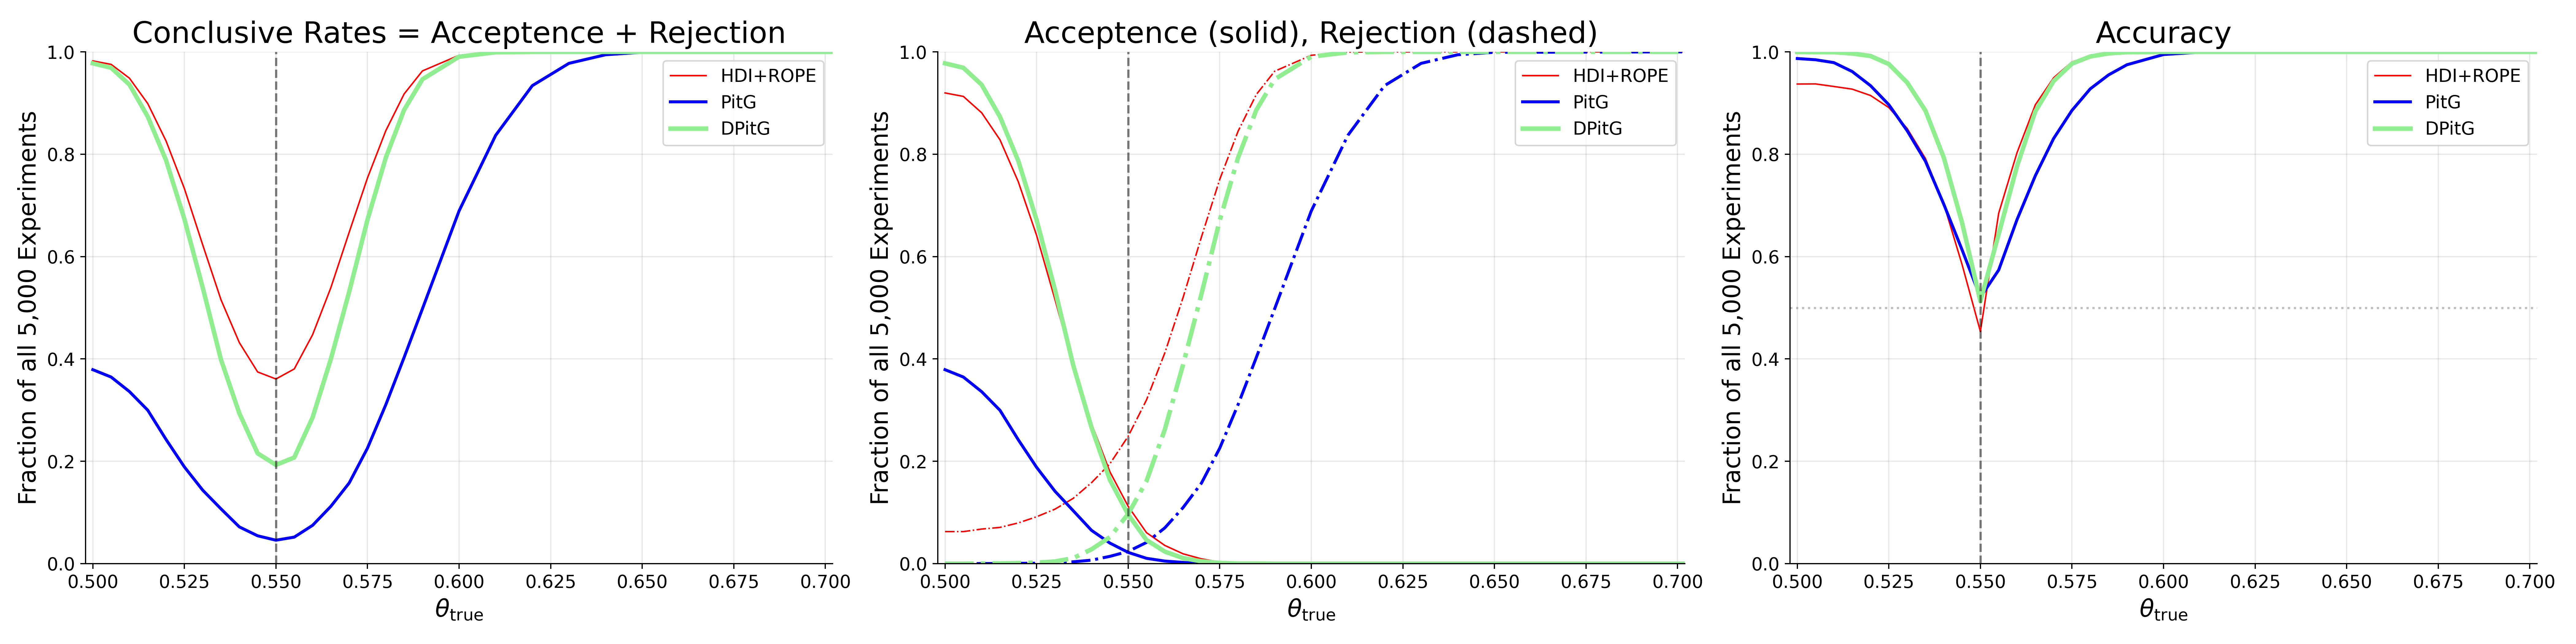
\includegraphics[width=1\textwidth]{conclusive_accuracy_rates_dpi350.png}
  \caption{Algorithm comparison across $\theta_{\rm true}$ values for $M=5{,}000$
  experiments ($\theta_{\rm null}=0.5$, $\omega_{\rm goal}=0.08$).
  \textit{Colors}: red: HDI+ROPE; blue: PitG; green: DPitG.
  \textit{Vertical dashed lines}: ${\rm ROPE}_{\rm max}=0.55$.
  \textit{Left}: conclusiveness rates.
  \textit{Middle}: acceptance (solid lines) and rejection (dashed lines) rates;
  at each $\theta_{\rm true}$ their sum equals the respective conclusiveness rate.
  \textit{Right}: accuracy rates (proportion of correct decisions out of all
  $M$ experiments); inconclusive experiments are assigned a decision based on whether
  $\hat{\theta}$ falls inside or outside the ROPE.}
  \label{fig:conclusiveness_rates}
\end{figure}

The left panel of Figure \ref{fig:conclusiveness_rates} shows that all three algorithms show a dip in conclusiveness as $\theta_{\rm true}$ approaches
${\rm ROPE}_{\rm max}$, after which conclusiveness rises again. The HDI+ROPE algorithm and DPitG
recover to near 100\% by $\theta_{\rm true}=0.6$; PitG only asymptotes to 100\% at
$\theta_{\rm true}\approx 0.64$, at which point DPitG and PitG become effectively
equivalent (for $\theta_{\rm null}=0.5$).

The precision-based methods are deliberately conservative near the ROPE boundaries,
yielding lower conclusiveness rates than the HDI+ROPE algorithm in this region; at ${\rm ROPE}_{\rm max}$
itself, DPitG is conclusive in only 19\% of experiments and PitG in only 5\%.
This dip is a natural consequence of the Decision Rule
(see Section~\ref{sec:accept_reject_meaning}): the ROPE boundaries are exactly the region
where neither an accept nor a reject verdict is easily justified.

Breaking the conclusiveness into its acceptance and rejection components (middle panel of Figure \ref{fig:conclusiveness_rates})
reveals the error structure.
For $\theta_{\rm null}=0.5$, acceptance is the correct decision within the ROPE
($\theta_{\rm true}\le 0.55$) and rejection is correct outside it.
The HDI+ROPE algorithm's false-reject rate climbs from $\sim\!6\%$ at $\theta_{\rm true}=0.5$
to $\sim\!30\%$ at ${\rm ROPE}_{\rm max}$; its false-accept rate peaks at
$\sim\!10\%$ at the ROPE boundary before dropping to $0\%$ by
$\theta_{\rm true}=0.57$. Both precision-based methods maintain a near-zero false-reject rate throughout:
exactly zero well within the ROPE interior, rising to a small level near the boundary:
DPitG reaching $\sim\!10\%$, and PitG lower only because its
conclusiveness rate is much smaller there.
Both also have false-accept rates that mirror the false-reject rates around
the ROPE boundary, which drops quickly as $\theta_{\rm true}$ moves outside.

The right panel of Figure \ref{fig:conclusiveness_rates} shows overall \textit{accuracy}, the proportion of correct decisions
across all $M$ experiments. Since the three algorithms have different conclusiveness
rates, inconclusive experiments must be assigned a decision for comparison.
We adopt the natural default: accept if $\hat{\theta}$ lies within the ROPE, reject
otherwise, the rule a practitioner would apply informally using the point estimate
alone, and the most common approach in empirical settings where credible intervals are
not examined; a more critical treatment of alternative imputation rules is deferred
to future work.

All three algorithms reach their minimum accuracy at ${\rm ROPE}_{\rm max}$. Within
the ROPE, DPitG consistently leads PitG, reaching 99.5\% at $\theta_{\rm true}=0.5$
compared to PitG's 98.5\%. Outside the ROPE, the HDI+ROPE algorithm and DPitG reach 100\% by
$\theta_{\rm true}=0.58$, whereas PitG achieves this only at
$\theta_{\rm true}\approx 0.60$.

That the HDI+ROPE algorithm reaches 100\% accuracy at $\theta_{\rm true}=0.58$ despite
producing biased $\hat{\theta}$ estimates motivates a closer look at the observed
sample proportion statistics. Figure~\ref{fig:success_by_truth_conclusive} shows, for
conclusive experiments, the IQR of $\hat{\theta}(N_{\rm stop})$ (left panel) and the
median bias $\hat{\theta}_{\rm 50\%}-\theta_{\rm true}$ (right panel).\footnote{We find
similar trends for the mean, but omit it to reduce clutter.}

As discussed in Section~\ref{sec:accept_reject_meaning}, accept/reject decisions rest on
the HDI's position relative to the ROPE, not on $\hat{\theta}$; a bias in $\hat{\theta}$
does not invalidate the decision so long as the HDI falls cleanly within (or outside)
the ROPE.


\begin{figure}[h!]
  \centering
  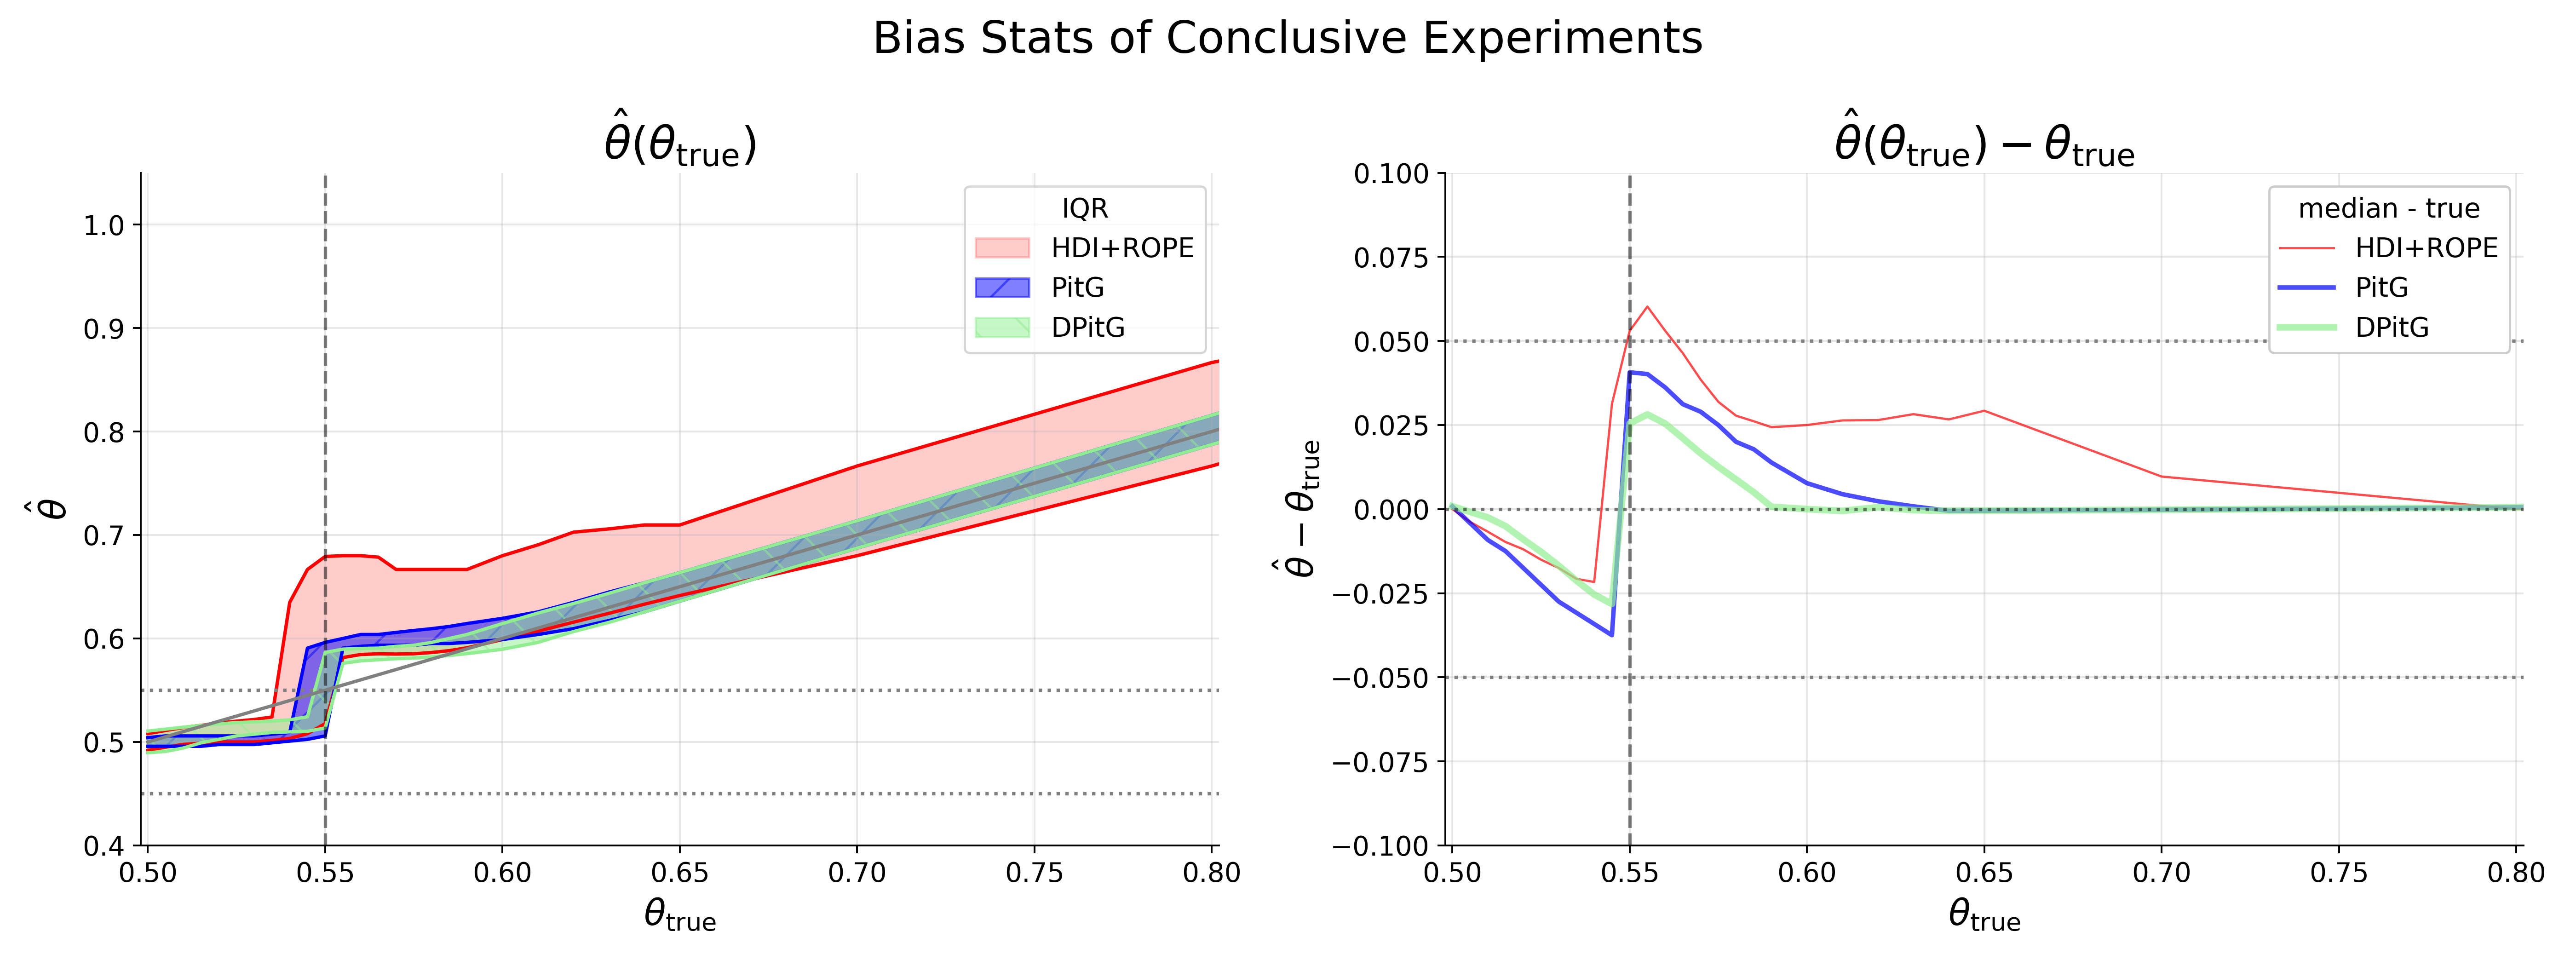
\includegraphics[width=1\textwidth]{success_by_truth_conclusive_dpi350.png}
  \caption{Sample proportion $\hat{\theta}(N_{\rm stop})$ at the stop iteration as a
  function of $\theta_{\rm true}$, for conclusive experiments only (subsets of $M=5{,}000$,
  $\theta_{\rm null}=0.5$, $\omega_{\rm goal}=0.08$, $N_{\rm min}=30$).
  \textit{Colors}: red: HDI+ROPE; blue: PitG; green: DPitG.
  \textit{Horizontal dotted lines}: ROPE boundaries.
  \textit{Vertical dashed line}: ${\rm ROPE}_{\rm max}$.
  \textit{Left}: interquartile range $\hat{\theta}_{\rm 25\%}$--$\hat{\theta}_{\rm 75\%}$
  of $\hat{\theta}(N_{\rm stop})$.
  \textit{Diagonal line}: parity line $\hat{\theta}=\theta_{\rm true}$.
  \textit{Right}: median bias $\hat{\theta}_{\rm 50\%}-\theta_{\rm true}$.}
  \label{fig:success_by_truth_conclusive}
\end{figure}

The HDI+ROPE algorithm's $\hat{\theta}$ bias is therefore more telling as a symptom of its lack of a
precision requirement than as a decision-quality metric. At $\theta_{\rm true}=0.5$,
all three algorithms show zero bias, as expected from the symmetry of the fair coin
case. Once $\theta_{\rm true}$ deviates from $0.5$, the HDI+ROPE algorithm's bias grows markedly: its
median bias approaches ${\rm ROPE}_{\rm max}$, with the upper
IQR extending substantially further, because the HDI+ROPE algorithm can stop on skewed samples before
sufficient data have accumulated to constrain the posterior.

The precision-based methods exhibit substantially smaller $\hat{\theta}$ bias, well
within the ROPE width across all $\theta_{\rm true}$ values, as a natural consequence
of their precision requirement. Among conclusive experiments within the ROPE, PitG
shows higher bias than DPitG; for inconclusive experiments (not shown\footnote{Bias
statistics for inconclusive experiments and the pooled analysis are available in the
open-source materials.}) (where PitG contributes far more cases than DPitG)
the pattern reverses, PitG's bias being slightly lower.
Pooled across both subsets, the aggregate difference is negligible: both methods yield
near-zero bias at all $\theta_{\rm true}$ values, with DPitG's aggregate bias only
marginally higher than PitG's.
Despite this, DPitG decision accuracy exceeds PitG's at every $\theta_{\rm true}$ value
(cf.\ Figure~\ref{fig:conclusiveness_rates}, right panel), because its substantially
higher conclusiveness rate more than compensates.

DPitG is decisively superior to PitG near and within the ROPE, at the cost of a larger
median $N_{\rm stop}$; having characterised the estimation properties of that superiority,
we now quantify its sampling cost.
Figure~\ref{fig:stop_iterations_by_truth_conclusive} quantifies $N_{\rm stop}$ for all three
algorithms, restricting to conclusive outcomes since inconclusive experiments always stop
at $N_{\rm max}$ and their stop iteration therefore carries no information about
algorithm behaviour; including the HDI+ROPE algorithm also illustrates why the precision
requirement matters.

\begin{figure}[h!]
  \centering
  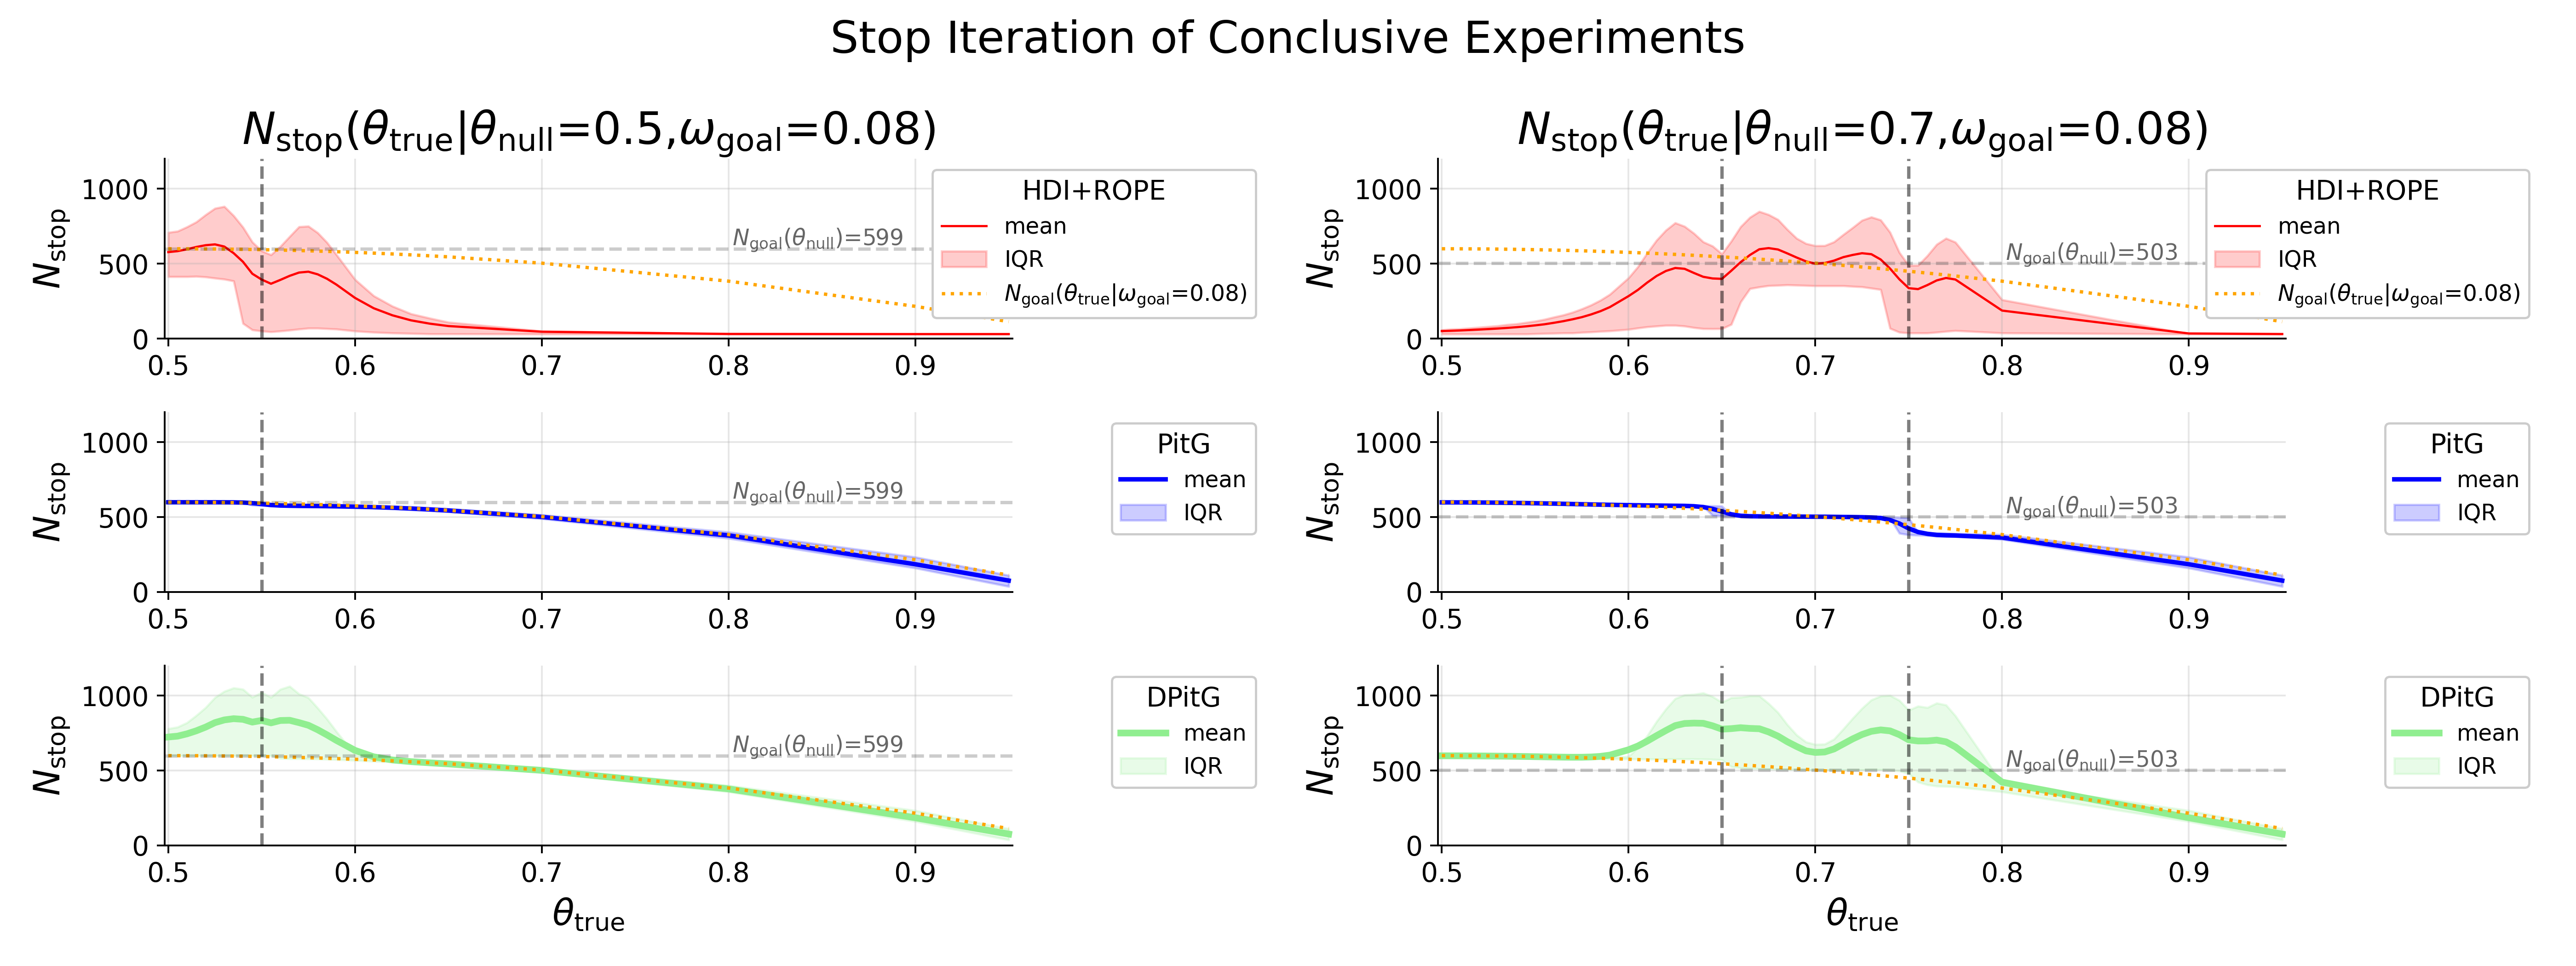
\includegraphics[width=1\textwidth]{stop_iterations_by_truth_conclusive_dpi350.png}
  \caption{Stop iteration $N_{\rm stop}$ statistics for conclusive experiments across
  $\theta_{\rm true}$ values ($\omega_{\rm goal}=0.08$).
  \textit{Left}: $\theta_{\rm null}=0.5$; \textit{Right}: $\theta_{\rm null}=0.7$.
  In each column the top, middle, and bottom panels correspond to HDI+ROPE, PitG,
  and DPitG, respectively.
  \textit{Band}: interquartile range $N_{\rm 25\%}$--$N_{\rm 75\%}$ of $N_{\rm stop}$.
  \textit{Solid line}: median $N_{\rm 50\%}$.
  \textit{Dotted line}: true precision-goal iteration
  $N_{\rm goal}(\theta_{\rm true}, \omega_{\rm goal})$ (Equation~\ref{eq:pitg_stop_iteration}).
  \textit{Horizontal dashed line}: null precision-goal iteration
  $N_{\rm goal}(\theta_{\rm null}, \omega_{\rm goal})$, the researcher's planned sample size.}
  \label{fig:stop_iterations_by_truth_conclusive}
\end{figure}

The HDI+ROPE algorithm shows distinctly different behaviour inside and outside the ROPE.
Within the ROPE, $N_{\rm stop}$ loosely tracks $N_{\rm goal}(\theta_{\rm true})$, but
with a wide IQR reflecting the absence of a precision criterion.
Right at ${\rm ROPE}_{\rm max}$, a distinctive V-shaped signature is visible:
$N_{\rm stop}$ dips to a narrow trough at the boundary, as the few conclusive
experiments there stop early by catching a chance excursion of the HDI just outside
the ROPE. 
Outside the ROPE, $N_{\rm stop}$ falls well below $N_{\rm goal}(\theta_{\rm true})$:
The HDI+ROPE algorithm correctly
rejects $\theta_{\rm null}$ much faster than precision-based methods, but does so on
the basis of imprecise posteriors, producing the strong $\hat{\theta}$ bias
(cf.\ Figure~\ref{fig:success_by_truth_conclusive}).

PitG stops tightly around $N_{\rm goal}(\theta_{\rm true})$ by design, making it the
natural reference for understanding the precision cost. The contrast with the planned
quantity $N_{\rm goal}(\theta_{\rm null})$ reveals an important asymmetry: because
$N_{\rm goal}(\theta)$ is maximised at $\theta=0.5$ and decreases as $\theta$ moves
towards $0$ or $1$, the direction of the gap depends on where $\theta_{\rm true}$ lies
relative to $\theta_{\rm null}$.

For $\theta_{\rm null}=0.5$, any deviation of $\theta_{\rm true}$ from $0.5$ implies
$N_{\rm goal}(\theta_{\rm true}) < N_{\rm goal}(\theta_{\rm null})$: the expected stop
iteration of $N_{\rm goal}=599$ is a conservative upper bound on $N_{\rm stop}$,
and experiments stop earlier whenever the truth differs from the null.

The right column of Figure~\ref{fig:stop_iterations_by_truth_conclusive} shows what
happens when the null does not coincide with the precision maximum.
The case $\theta_{\rm null}=0.7$ is representative of a researcher expecting an elevated
base rate (such as a presumed 70\% success probability for an established treatment)
who must judge whether the true rate is practically equivalent to that benchmark.
Unlike the fair coin case, where $\theta_{\rm null}=0.5$ maximises $\theta(1-\theta)$
so any deviation of $\theta_{\rm true}$ reduces the required sample, here the symmetry
breaks: the same deviation can either reduce or increase $N_{\rm goal}$ depending on
its direction.

In particular, when $\theta_{\rm true}<\theta_{\rm null}$ (moving closer to $0.5$),
$N_{\rm goal}(\theta_{\rm true})>N_{\rm goal}(\theta_{\rm null}=0.7)\approx 503$:
the planned budget underestimates the samples required, and
$N_{\rm goal}(\theta_{\rm null})$ acts as a lower bound rather than an upper
one.\footnote{When $\theta_{\rm true}>\theta_{\rm null}=0.7$ (moving further from
$0.5$), $N_{\rm goal}(\theta_{\rm true})<N_{\rm goal}(\theta_{\rm null})$ and
experiments stop sooner than planned.
The PitG median stop iteration visibly exceeds $N_{\rm goal}(\theta_{\rm null})=503$
for $\theta_{\rm true}<0.7$, confirming this underestimate.
DPitG shows qualitatively similar patterns to the $\theta_{\rm null}=0.5$ column
near both ROPE boundaries, elevated above $N_{\rm goal}(\theta_{\rm true})$ where
the conclusiveness gain is largest.}

In general, $N_{\rm goal}(\theta_{\rm null})$ serves as the researcher's advance
planning estimate: a conservative upper bound when $\theta_{\rm null}$ lies at the
precision maximum (e.g.\ $\theta_{\rm null}=0.5$), and a floor otherwise.
The researcher should set $N_{\rm max}$ according to their resources, with
$N_{\rm goal}(\theta_{\rm null})$ as the baseline (here $N_{\rm max}=1{,}500$).

DPitG's $N_{\rm stop}$ equals or exceeds PitG's within the ROPE and in the vicinity
of its boundaries, the extra iterations being precisely what accounts for the higher
conclusiveness seen in Figure~\ref{fig:conclusiveness_rates}. Once $\theta_{\rm true}$
is far enough from the ROPE, DPitG converges to PitG and both stop at
$N_{\rm goal}(\theta_{\rm true})$.

Figure~\ref{fig:stop_conclusiveness_ratios} places the DPitG--PitG trade-off in direct
comparison by overlaying the ratio of conclusiveness rates
(from Figure~\ref{fig:conclusiveness_rates}) and the ratio of $N_{\rm stop}$
(from Figure~\ref{fig:stop_iterations_by_truth_conclusive}) across $\theta_{\rm true}$.\footnote{The
apparent flattening of the stop iteration ratio near ${\rm ROPE}_{\rm max}$ is an artefact of
the finite cap $N_{\rm max}=1{,}500$; with a larger cap both curves would peak sharply
at the boundary.}


\begin{figure}[h!]
  \centering
  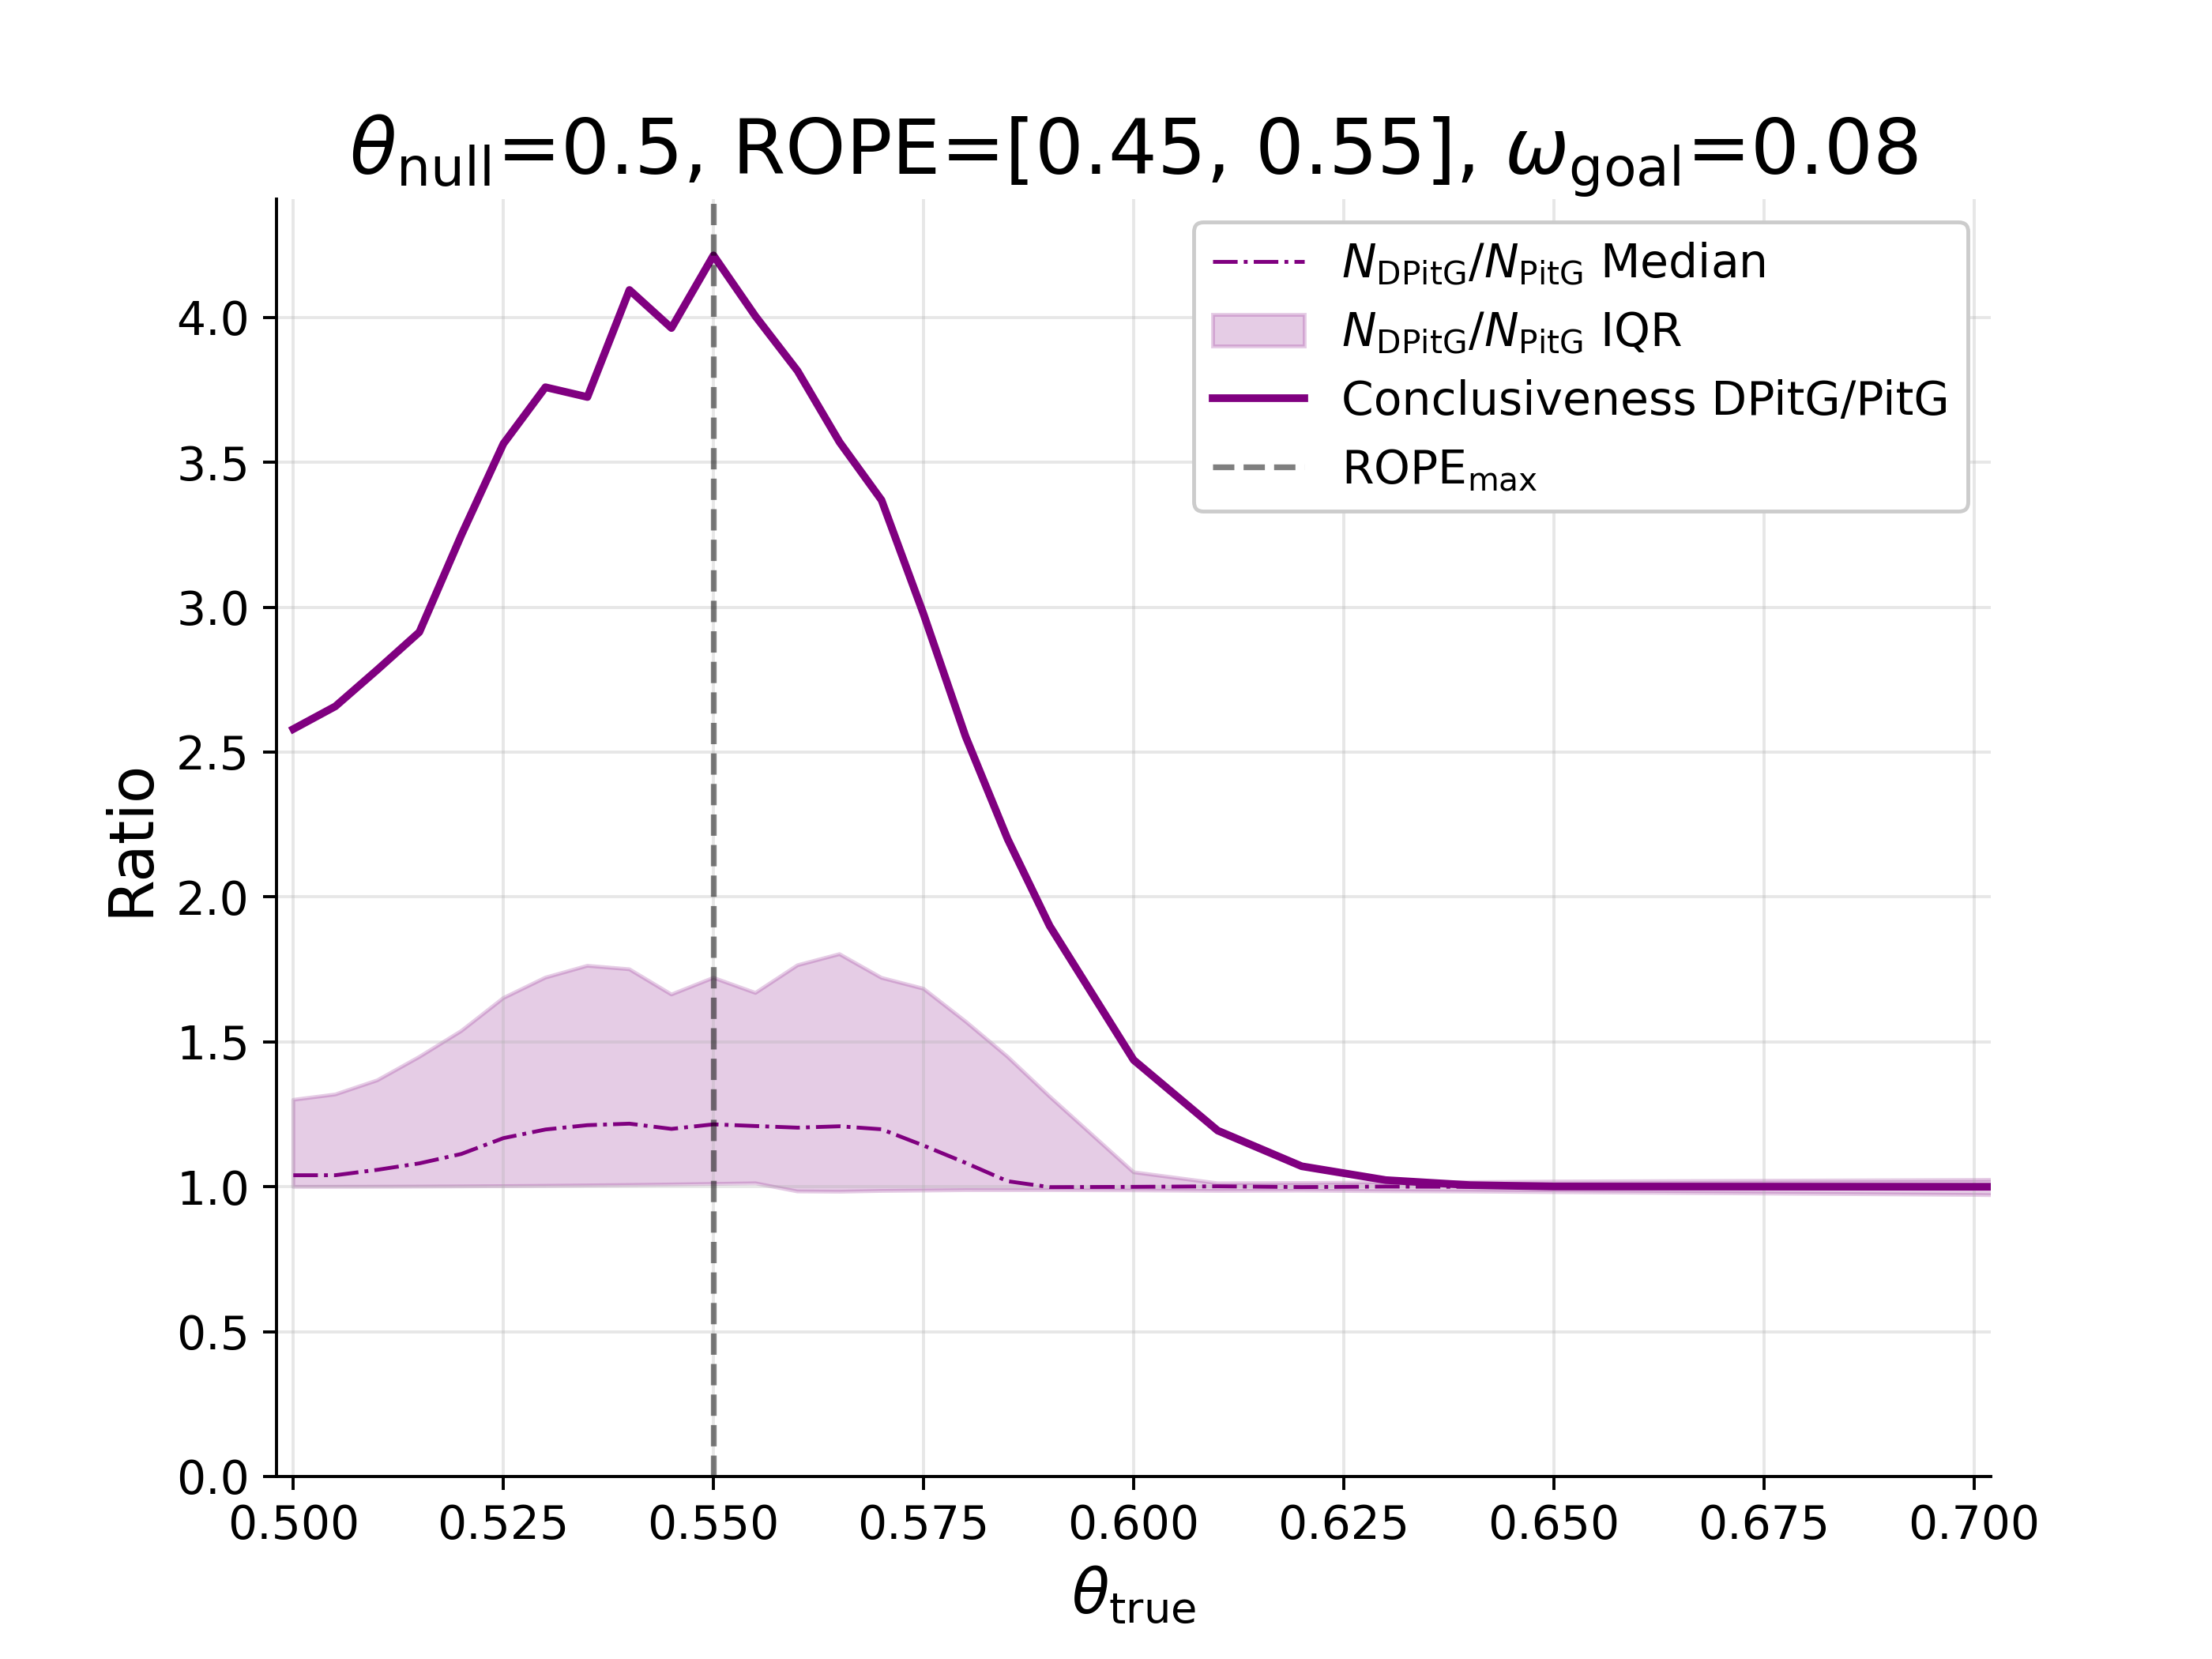
\includegraphics[width=1\textwidth]{stop_conclusiveness_ratios_dpi350.png}
  \caption{DPitG-to-PitG ratios of conclusiveness rate and stop iteration across
  $\theta_{\rm true}$ values ($M=5{,}000$, $\theta_{\rm null}=0.5$,
  $\omega_{\rm goal}=0.08$).
  \textit{Solid line}: conclusiveness ratio
  (cf.\ Figure~\ref{fig:conclusiveness_rates}).
  \textit{Dot-dashed line}: median $N_{\rm stop}$ ratio.
  \textit{Band}: interquartile range of the $N_{\rm stop}$ ratio.
  \textit{Vertical dashed line}: ${\rm ROPE}_{\rm max}=0.55$.}
  \label{fig:stop_conclusiveness_ratios}
\end{figure}

The conclusiveness ratio substantially exceeds the $N_{\rm stop}$ ratio throughout,
particularly within and near the ROPE.
Strikingly, the conclusiveness ratio remains above 1 even where the $N_{\rm stop}$
ratio approaches 1 (roughly $0.60 \lesssim \theta_{\rm true} \lesssim 0.63$), confirming
that DPitG gains conclusive outcomes at negligible extra sampling cost in this region.
The lower IQR band confirms that a substantial fraction of DPitG experiments stop
exactly when PitG does.
The fair coin quantitative summary (a $2.6\times$ conclusiveness gain at a median
$4\%$ sampling premium) is consistent with Table~\ref{tab:fair_overall} and
Section~\ref{sec:fair_coin_large_scale}; Table~\ref{tab:goal_impact} shows how the
conclusiveness ratio varies with $\omega_{\rm goal}$.


The DPitG advantage documented here generalises: qualitatively similar conclusiveness
gains hold for $\theta_{\rm null}=0.7$ (as shown in the right panel of
Figure~\ref{fig:stop_iterations_by_truth_conclusive}) and across $\omega_{\rm goal}$
values (see Section~\ref{sec:goal_impact} for the fair coin case).
